\documentclass[article]{jss}
\usepackage[utf8]{inputenc}

\providecommand{\tightlist}{%
  \setlength{\itemsep}{0pt}\setlength{\parskip}{0pt}}

\author{
Anna Michalek\\European Central Bank \And Alain Quartier-la-Tente\\Insee
}
\title{\pkg{RJDemetra}: A R Interface To JDemetra+ Seasonal Adjustment Software}

\Plainauthor{Anna Michalek, Alain Quartier-la-Tente}
\Plaintitle{\pkg{RJDemetra}: A R Interface To JDemetra+ Seasonal Adjustment Software}
\Shorttitle{\pkg{RJDemetra}: A R Interface To JDemetra+ Seasonal Adjustment Software}

\Abstract{
The abstract of the article.
}

\Keywords{\proglang{R}, seasonal adjustment, calendar effects, ARIMA, time series}
\Plainkeywords{R, seasonal adjustment, calendar effects, ARIMA, time series}

%% publication information
%% \Volume{50}
%% \Issue{9}
%% \Month{June}
%% \Year{2012}
%% \Submitdate{}
%% \Acceptdate{2012-06-04}

\Address{
    }

% Pandoc header

\usepackage{amsmath} \usepackage{booktabs} \usepackage{longtable} \usepackage{array} \usepackage{multirow} \usepackage{wrapfig} \usepackage{float} \usepackage{pdflscape} \usepackage{tabu} \usepackage{threeparttable} \usepackage{threeparttablex} \usepackage[normalem]{ulem} \usepackage{makecell}

\begin{document}

\hypertarget{introduction}{%
\section{Introduction}\label{introduction}}

Since the 20th century, more and more infra-annual statistics are
produced, especially by national institutes, to analyse the short-term
evolution of an economy. It is for example the case of the gross
domestic product (GDP), unemployment rate, household consumption of
goods and industrial production indices. However, most of those time
series are affected by seasonal and trading days effects. A seasonal
effect is an effect that occur in the same calendar month with similar
magnitude and direction from year to year. For instance, automobile
production is usually lower during summer, due to holidays, and
chocolate sales are usually higher in December, due to Christmas.
Trading days effect is the fact that a time series can be affected by
each calendar month's weekday composition. For example retail sales are
usually higher on Saturday, thus they are likely to be higher in months
with a surplus of weekend days.

Therefore, seasonal and trading days effects can make it difficult to
analyse the infra-annual movements of a time series or to make spatial
comparison. That's why time series are often seasonally and trading days
adjusted and seasonal adjustment is the process of removing the effects
of seasonal and trading day fluctuations.

The most popular seasonal adjustment methods are TRAMO-SEATS+\footnote{The
  program TRAMO-SEATS+ was developed by Gianluca Caporello and Agustin
  Maravall --- with programming support from Domingo Perez and Roberto
  Lopez --- at the Bank of Spain. It is based on the program
  TRAMO-SEATS, previously developed by Victor Gomez and Agustin
  Maravall.} \citep{gomez1996programs, caporello2004program}, a
parametric method based on ARIMA models, and X-13-ARIMA-SEATS\footnote{The
  program X-13ARIMA-SEATS is a produced, distributed, and maintained by
  the US-Census Bureau.} \citep{findleyx12, ladiray1999x11en}, a
non-parametric method based on moving average. Both methods are
recommended by Eurostat and the European Central Bank (ECB) to
seasonnaly adjust economic indicators. These methods proceed in two
steps summarized in figure \ref{fig:2_step_proc}.

\begin{figure}[htb]
\centering
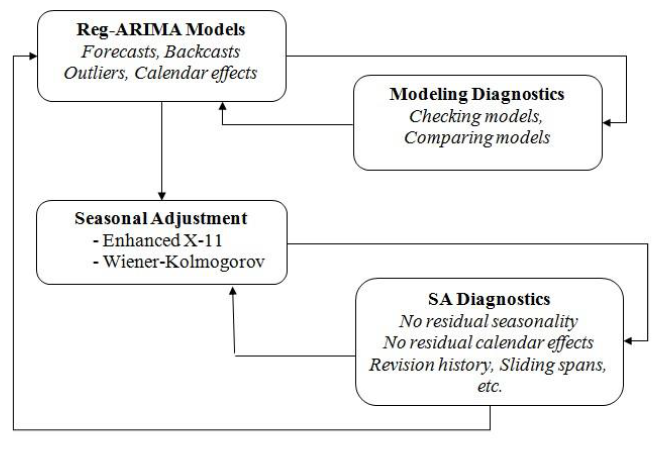
\includegraphics[scale=0.8]{img/sa_2_steps.PNG} 
\caption{X-13-ARIMA-SEATS and TRAMO-SEATS+ 2-step process: pre-adjustment and decomposition.}
\label{fig:2_step_proc}
\end{figure}

The \textbf{first step} of seasonal adjustment consists of pre-adjusting
the time series by removing from it the deterministic effects and
estimating missing observations. Among deterministic effects, we
distinguish outliers, calendar and regression effects. In this step,
also forecasts and backcasts of the pre-adjusted series are estimated
which allows applying linear filters at both ends of the series in the
second step of the seasonal adjustment. The pre-adjustment,
linearization, of the input series is achieved with a \textbf{RegARIMA}
model (model with ARIMA errors) as specified below.

\[z_t=y_t\beta+x_t\] where

\begin{itemize}
\tightlist
\item
  \(z_t\) - is the original series;
\item
  \(\beta = (\beta_1,\dots,\beta_n)\) - a vector of regression
  coefficients;
\item
  \(y_t = (y_{1t},\dots,y_{nt})\) - \(n\) regression variables
  (outliers, calendar effects, user-defined variables);
\item
  \(x_t\) - a disturbance that follows the general ARIMA process:
\item
  \(\phi(B)\delta(B)x_t=\theta(B)a_t\); \(\phi(B), \delta(B)\) and
  \(\theta(B)\) are the finite polynomials in \(B\); \(a_t\) is a
  white-noise variable with zero mean and a constant variance.
\end{itemize}

The polynomial \(\phi(B)\) is a stationary autoregressive (AR)
polynomial in \(B\), which is a product of the stationary regular AR
polynomial in \(B\) and the stationary seasonal polynomial in \(B^s\):

\[\phi(B)=\phi_p(B)\Phi_{bp}(B^s)=(1+\phi_1B+\dots+\phi_pB^p)(1+\Phi_1B^s+\dots+\Phi_{bp}B^{bps}\]

where:

\begin{itemize}
\tightlist
\item
  \(p\) - number of regular AR terms (in the package and in JDemetra+
  \(p \le 3\));
\item
  \(bp\) - number of seasonal AR terms (in the package and in JDemetra+
  \(bp \le 1\));
\item
  \(s\) - number of observations per year (frequency of the time
  series).
\end{itemize}

The polynomial \(\theta(B)\) is an invertible moving average (MA)
polynomial in \(B\), which is a product of the invertible regular MA
polynomial in \(B\) and the invertible seasonal MA polynomial in
\(B^s\):

\[\theta(B)=\theta_q(B)\Theta_{bq}(B^s)=(1+\theta_1B+\dots+\theta_qB^q)(1+\Theta_1B^s+\dots+\Theta_{bq}B^{bqs})\]

where:

\begin{itemize}
\tightlist
\item
  \(q\) - number of regular MA terms (in the package and in JDemetra+
  \(q \le 3\));
\item
  \(bq\) - number of seasonal MA terms (in the package and in JDemetra+
  \(bq \le 1\));
\end{itemize}

The polynomial \(\delta(B)\) is the non-stationary AR polynomial in
\(B\) (unit roots):

\[\delta(B)=(1-B)^d(1-B^s)^{d_s}\]

where:

\begin{itemize}
\tightlist
\item
  \(d\) - regular differencing order (in the package and in JDemetra+
  \(d \le 1\));
\item
  \(d_s\) - seasonal differencing order (in the package and in JDemetra+
  \(d_s \le 1\));
\end{itemize}

An automatic modelling is also implemented in both methods to: determine
the decomposition of the series, detect outliers and calendar effects
and to adjust residuals to an ARIMA models. A detailed description can
be found in \cite{gomez1998automatic}.

In the \textbf{second part} of seasonal adjustment, called the
\textbf{decomposition}, the pre-adjusted series (\(y\)) is decomposed
into the following components: trend-cycle (\(t\)), seasonal component
(\(s\)) and irregular component (\(i\)). The decomposition can be:

\begin{itemize}
\tightlist
\item
  additive (\(y = t + s + i\))\\
\item
  multiplicative (\(y = t * s * i\))\\
\item
  log-additive (\(\log(y) = \log(t) + \log(s) + \log(i)\)) or\\
\item
  pseudo-additive (\(y = t * (s + i - 1)\))
\end{itemize}

The method of decomposing the pre-adjusted series differs between
TRAMO-SEATS+ and X-12ARIMA/X-13ARIMA. In TRAMO-SEATS+, SEATS (Signal
Extraction in ARIMA Time Series) decomposes the observed series with a
ARIMA-model based method
\citep{gomez1996programs, caporello2004program}. Whereas in
X-12ARIMA/X-13ARIMA, the X-11 algorithm decomposes the time series by
means of linear filters \citep{findleyx12, ladiray1999x11en}.

As a result of seasonal adjustment, the final seasonally adjusted series
shall be free of seasonal and calendar-related movements.

\hypertarget{jdemetra-and-rjdemetra}{%
\section{JDemetra+ and RJDemetra}\label{jdemetra-and-rjdemetra}}

JDemetra+ is a new tool for seasonal adjustment (SA) developed by the
National Bank of Belgium (NBB) in cooperation with the Deutsche
Bundesbank and Eurostat in accordance with the Guidelines of the
European Statistical System (ESS) \citep{eurostat2015guidelines}. It
implements the concepts and algorithms used in the two leading SA
methods: TRAMO-SEATS+ and X-12ARIMA/X-13ARIMA-SEATS. Those methods have
been re-engineered using an object-oriented approach that enables easier
handling, extensions and modifications.

JDemetra+ has been
\href{https://ec.europa.eu/eurostat/cros/system/files/Jdemetra_\%20release.pdf}{officially
recommended}, since 2 February 2015, to the members of the ESS and the
European System of Central Banks as software for seasonal and calendar
adjustment of official statistics.

Besides seasonal adjustment, JDemetra+ bundles other time series models
that are useful in the production or analysis of economic statistics,
including for instance outlier detection, nowcasting, temporal
disaggregation or benchmarking. More details on the methodology used in
JDemetra+ can be found in the JDemetra+ manuals and user guides
\citep{grudkowska2015jdemetrarm, grudkowska2015jdemetraug}.

The package \pkg{RJDemetra} provides a R interface to the seasonal
adjustment software JDemetra+. \pkg{RJDemetra} uses Java libraries of
JDemetra+, thus it relies on the \pkg{rJava} \citep{rJava} package and
Java SE 8 or later version is required. It allows to:

\begin{itemize}
\tightlist
\item
  perform seasonal adjustment with TRAMO-SEATS+ and
  X-12ARIMA/X-13ARIMA-SEATS with pre-defined (section \ref{pre-def-est})
  and user-defined specification (section \ref{user-def-spec});\\
\item
  acces to all the output available in JDemetra+ (section
  \ref{sa-obj-struc});\\
\item
  import and export JDemetra+ workspaces (section
  \ref{manipulate-workspace}).
\end{itemize}

It can be installed from CRAN:

\begin{CodeChunk}

\begin{CodeInput}
R> install.packages("RJDemetra")
\end{CodeInput}
\end{CodeChunk}

The development version can be installed from GitHub with \pkg{devtools}
\citep{devtools}:

\begin{CodeChunk}

\begin{CodeInput}
R> devtools::install_github("jdemetra/rjdemetra")
\end{CodeInput}
\end{CodeChunk}

\hypertarget{dataset}{%
\subsection{Dataset}\label{dataset}}

In this package the sts\_inpr\_m database of Eurostat is included, which
contains monthly industrial production indices in manufacturing in the
European Union. It contains 37 time series from january 1990 to december
2017 which are considered to be affected by seasonal and trading days
effects. The data is a \code{ts} object and can be accessed using the
\code{ipi_c_eu} object. The following snippet of code plots the
industrial production index of the euro aera (EA19):

\begin{CodeChunk}

\begin{CodeInput}
R> library(RJDemetra)
R> plot(ipi_c_eu[, "EA19"])
\end{CodeInput}


\begin{center}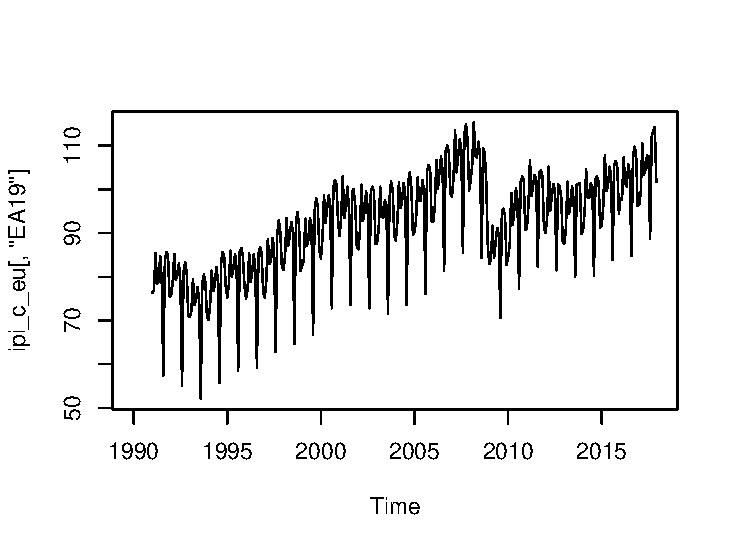
\includegraphics{img/img-basic_raw_data_plot-1} \end{center}

\end{CodeChunk}

\hypertarget{print-styling}{%
\subsection{Print styling}\label{print-styling}}

By default, a color styling is used for the \code{print} methods of the
objects created by \pkg{RJDemetra}. It can causes troubles with some
outputs (for example with \pkg{rmarkdown} \citep{rmarkdown}) and can be
disabled in each \code{print} function with the argument
\code{enable_print_style = FALSE} or setting the global option
\code{enable_print_style} to \code{FALSE}:

\begin{CodeChunk}

\begin{CodeInput}
R> options(enable_print_style = FALSE)
\end{CodeInput}
\end{CodeChunk}

\hypertarget{pre-def-est}{%
\section{Estimate a pre-defined RegARIMA and SA
model}\label{pre-def-est}}

As in JDemetra+, \pkg{RJDemetra} allows to perform seasonal adjustment
using pre-defined model specifications. The pre-defined specifications
correspond to most commonly used specifications and users are
recommended to start their analysis with one of them. They are
separately defined for TRAMO-SEATS and X-13ARIMA-SEATS estimation
methods. It is also possible to perform only the first step of seasonal
adjustment (the RegARIMA estimation). The pre-defined model
specifications are described in tables \ref{tab:pre_def_ts} and
\ref{tab:pre_def_x13}. They are identical for pre-adjustment (column 1)
and for seasonal adjustment (column 2). With more details, setting
described in tables tables \ref{tab:pre_def_ts} and
\ref{tab:pre_def_x13} are:

\begin{itemize}
\tightlist
\item
  Transformation test: a test to choose between an additive
  decomposition (no transformation) and a multiplicative decomposition
  (logarithmic transformation).\\
\item
  Pre-adjustment for leap-year: in the case of a multiplicaive
  decomposition; a correction of the February values is applied to the
  original series (before transformation). The original values in
  February are multiplied by \(\frac{28.25}{29}\) for leap years, by
  \(\frac{28.25}{28}\) for non-leap years and values for other months
  are not modified. In the case of multiplicative models, this is
  equivalent to adding a leap year regressor
  \citep{bell1992lengthmonthadj}.
\item
  Working days: a pre-test is made for a presence of a working day
  effect.\\
\item
  Trading days: a pre-test is made for a presence of a trading day
  effect.\\
\item
  Easter: a pre-test for a presence of the Easter effect. The default
  length of the Easter effect is 6 days (for TRAMO-SEATS specifications)
  and 8 days (for X-13ARIMA-SEATS specifications).\\
\item
  Outliers: an automatic identification of three types of outliers: AO
  (additive outlier), LS (level shift) and TC (transitory change), using
  a default critical value. The automatic identification of SO (seasonal
  outlier) is not enabled by default.
\item
  ARIMA model: the choice between fixing the ARIMA model structure to
  (0,1,1)(0,1,1) (Airline model) or searching for the ARIMA model using
  an automatic model identification procedure. The Airline model is used
  as a default model in several TRAMO-SEATS+ and X-13ARIMA-SEATS
  specifications because it has been shown in many studies that this
  model is appropriate for many real seasonal monthly or a quarterly
  time series. Moreover, the Airline model approximates well many other
  models and provides an excellent ``benchmark'' model
  \citep{maravall2009identification}.
\end{itemize}

\begin{table}[t]

\caption{\label{tab:pre_def_ts}Pre-defined specification for TRAMO and TRAMO-SEATS}
\centering
\fontsize{7}{9}\selectfont
\begin{tabular}{c>{\centering\arraybackslash}p{1.cm}>{\centering\arraybackslash}p{1.cm}>{\centering\arraybackslash}p{1.5cm}>{\centering\arraybackslash}p{0.9cm}>{\centering\arraybackslash}p{0.9cm}>{\centering\arraybackslash}p{1.5cm}>{\centering\arraybackslash}p{0.9cm}c}
\toprule
\multicolumn{2}{c}{Specification} & \multicolumn{1}{c}{} \\
\cmidrule(l{3pt}r{3pt}){1-2}
TRAMO & TRAMO-SEATS & Trans-formation & Pre-adjust-ment for leap-year & Working days & Trading days & Easter effect & Outliers & ARIMA model\\
\midrule
TR0 & RSA0 & no & no & no & no & no & no & (0,1,1)(0,1,1)\\
TR1 & RSA1 & test & no & no & no & no & test & (0,1,1)(0,1,1)\\
TR2 & RSA2 & test & no & test & no & test & test & (0,1,1)(0,1,1)\\
TR3 & RSA3 & test & no & no & no & no & test & AMI\\
TR4 & RSA4 & test & no & test & no & test & test & AMI\\
\addlinespace
TR5 & RSA5 & test & no & no & yes & test (Standard) & test & AMI\\
TRfull (default) & RSAfull (default) & test & yes & no & test & test (Include Easter) & test & AMI\\
\bottomrule
\end{tabular}
\end{table}

\begin{table}[t]

\caption{\label{tab:pre_def_x13}Pre-defined specification for RegARIMA and X-13ARIMA-SEATS}
\centering
\fontsize{7}{9}\selectfont
\begin{tabular}{c>{\centering\arraybackslash}p{1.7cm}>{\centering\arraybackslash}p{1.cm}>{\centering\arraybackslash}p{1.4cm}>{\centering\arraybackslash}p{0.9cm}>{\centering\arraybackslash}p{0.9cm}>{\centering\arraybackslash}p{0.9cm}>{\centering\arraybackslash}p{0.9cm}c}
\toprule
\multicolumn{2}{c}{Specification} & \multicolumn{1}{c}{} \\
\cmidrule(l{3pt}r{3pt}){1-2}
RegARIMA & X-13ARIMA-SEATS & Trans-formation & Pre-adjust-ment for leap-year & Working days & Trading days & Easter effect & Outliers & ARIMA model\\
\midrule
RG0 &  & no & no & no & no & no & no & (0,1,1)(0,1,1)\\
RG1 & RSA1 & test & no & no & no & no & test & (0,1,1)(0,1,1)\\
RG2c & RSA2c & test & test & test & no & test & test & (0,1,1)(0,1,1)\\
RG3 & RSA3 & test & no & no & no & no & test & AMI\\
RG4c & RSA4c & test & test & test & no & test & test & AMI\\
\addlinespace
RG5c (default) & RSA5 (default) & test & test & no & test & test & test & AMI\\
\bottomrule
\end{tabular}
\end{table}

Four functions can be used in \pkg{RJDemetra} to perform an estimation
with the pre-defined specification:

\begin{itemize}
\tightlist
\item
  RegARIMA

  \begin{itemize}
  \tightlist
  \item
    X-13ARIMA method: \code{regarima_def_x13()}
  \item
    TRAMO-SEATS method: \code{regarima_def_tramoseats()}
  \end{itemize}
\item
  Seasonal adjustment

  \begin{itemize}
  \tightlist
  \item
    X-13ARIMA method: \code{x13_def()}
  \item
    TRAMO-SEATS method: \code{tramoseats_def()}
  \end{itemize}
\end{itemize}

For examples:

\begin{CodeChunk}

\begin{CodeInput}
R> myseries <- ipi_c_eu[, "EA19"]
R> 
R> regx13 <- regarima_def_x13(myseries, spec = "RG5c")
R> regts <- regarima_def_tramoseats(myseries, spec = "TRfull")
R> sax13 <- x13_def(myseries, spec = "RSA3", userdefined = NULL)
R> sats <- tramoseats_def(myseries, spec = "RSAfull", userdefined = NULL)
\end{CodeInput}
\end{CodeChunk}

In section \ref{user-def-spec} it is presented how to modify model
specifications, including the possibility to incorprate user-defined
regressors.

\hypertarget{sa-obj-struc}{%
\section{Class object structure}\label{sa-obj-struc}}

In section \ref{pre-def-est} it was presented how to run a RegARIMA and
complete seasonal adjustment estimation with pre-defined model
specifications. In this section the outcome will be described in detail.

As a result of seasonal adjustment estimation (e.g.~function
\code {x13_def} or \code {tramoseats_def}) a S3 class object
(\code{sa_object}) is created. It has a class \code{c("SA","X13")} or
\code{c("SA","TRAMO_SEATS")} depending on the used estimation method.
The \code{sa_object} consist of lists of S3 class sub-objects. For each
of the class \code{print} and \code{plot} methods are defined. The
complete structure of the \code{sa_object} is presented in table
\ref{tab:obj_tab}. In general, the \code{sa_object} contains the
following five objects: \textbf{regarima}, \textbf{decomposition},
\textbf{final}, \textbf{diagnostics} and \textbf{user\_defined}.
Independently which of the two estimation methods is used the regarima,
final and diagnostics objects contain the same components, though with
different classes (see table \ref{tab:obj_tab}). Whereas, the object
decomposition differs for the two methods. The object user\_defined is
empty unless additional output was requested by the user (see
sub-section \ref{user-def}). Finally, when estimating RegARIMA only the
regarima object is created. All the plots methods are detailed in table
\ref{tab:plots_methods}.

\begingroup\fontsize{7}{9}\selectfont

\begin{longtable}{lllll}
\caption{\label{tab:obj_tab}SA object structure}\\
\toprule
\multicolumn{1}{c}{ } & \multicolumn{1}{c}{ } & \multicolumn{1}{c}{ } & \multicolumn{2}{c}{When adjusted with:} \\
\cmidrule(l{3pt}r{3pt}){4-5}
\multicolumn{1}{c}{\em{ }} & \multicolumn{1}{c}{\em{ }} & \multicolumn{1}{c}{\em{ }} & \multicolumn{1}{c}{\em{x13/x13\_def}} & \multicolumn{1}{c}{\em{ tramoseats/tramoseats\_def}} \\
\cmidrule(l{3pt}r{3pt}){4-4} \cmidrule(l{3pt}r{3pt}){5-5}
Object & Level & Type & Class & Class\\
\midrule
sa\_object & 0 & list & SA, X13 & SA, TRAMO\_SEATS\\
\textbf{\hspace{1em}regarima} & \textbf{1} & \textbf{list} & \textbf{regarima, X13} & \textbf{regarima, TRAMO\_SEATS}\\
\hspace{2em}specification & 2 & list &  & \\
\hspace{3em}estimate & 3 & data.frame &  & \\
\hspace{3em}transform & 3 & data.frame &  & \\
\addlinespace
\hspace{3em}regression & 3 & list &  & \\
\hspace{4em}userdef & 4 & list &  & \\
\hspace{5em}specification & 5 & data.frame &  & \\
\hspace{5em}outliers & 5 & data.frame or NA(empty) &  & \\
\hspace{5em}variables & 5 & list &  & \\
\addlinespace
\hspace{6em}series & 6 & mts, ts, matrix or NA(empty) &  & \\
\hspace{6em}description & 6 & data.frame or NA(empty) &  & \\
\hspace{4em}trading.days & 4 & data.frame &  & \\
\hspace{4em}easter & 4 & data.frame &  & \\
\hspace{3em}outliers & 3 & data.frame &  & \\
\addlinespace
\hspace{3em}arima & 3 & list &  & \\
\hspace{4em}specification & 4 & data.frame &  & \\
\hspace{4em}coefficients & 4 & data.frame or NA(empty) &  & \\
\hspace{3em}forecast & 3 & data.frame &  & \\
\hspace{3em}span & 3 & data.frame &  & \\
\addlinespace
\hspace{2em}arma & 2 & vector - numeric &  & \\
\hspace{2em}arima.coefficients & 2 & matrix &  & \\
\hspace{2em}regression.coefficients & 2 & matrix &  & \\
\hspace{2em}loglik & 2 & matrix &  & \\
\hspace{2em}model & 2 & list &  \vphantom{1} & \\
\addlinespace
\hspace{3em}spec\_rslt & 3 & data.frame &  & \\
\hspace{3em}effects & 3 & mts, ts, matrix &  & \\
\hspace{2em}residuals & 2 & ts &  & \\
\hspace{2em}residuals.stat & 2 & list &  & \\
\hspace{3em}st.error & 3 & numeric &  & \\
\addlinespace
\hspace{3em}tests & 3 & data.frame & regarima\_rtests, data.frame & \\
\hspace{2em}forecast & 2 & mts, ts, matrix &  & \\
\textbf{\hspace{1em}decomposition} & \textbf{1} & \textbf{list} & \textbf{decomposition\_X11} & \textbf{}\\
\hspace{2em}specification & 2 & data.frame & X11\_spec, data.frame & \\
\hspace{2em}mode & 2 & character &  \vphantom{1} & \\
\addlinespace
\hspace{2em}mstats & 2 & matrix &  & \\
\hspace{2em}si\_ratio & 2 & mts, ts, matrix &  & \\
\hspace{2em}s\_filter & 2 & vector - character &  & \\
\hspace{2em}t\_filter & 2 & character &  & \\
\textbf{\hspace{1em}decomposition} & \textbf{1} & \textbf{list} & \textbf{} & \textbf{decomposition\_SEATS}\\
\addlinespace
\hspace{2em}specification & 2 & data.frame & seats\_spec, data.frame & \\
\hspace{2em}mode & 2 & character &  & \\
\hspace{2em}model & 2 & list &  & \\
\hspace{3em}model & 3 & matrix or empty list &  & \\
\hspace{3em}sa & 3 & matrix or empty list &  & \\
\addlinespace
\hspace{3em}trend & 3 & matrix or empty list &  & \\
\hspace{3em}seasonal & 3 & matrix or empty list &  & \\
\hspace{3em}transitory & 3 & matrix or empty list &  & \\
\hspace{3em}irregular & 3 & matrix or empty list &  & \\
\hspace{2em}linearized & 2 & mts, ts, matrix &  & \\
\addlinespace
\hspace{2em}components & 2 & mts, ts, matrix &  & \\
\textbf{\hspace{1em}final} & \textbf{1} & \textbf{list} & \textbf{final} & \textbf{}\\
\hspace{2em}series & 2 & mts, ts, matrix &  & \\
\hspace{2em}forecasts & 2 & mts, ts, matrix &  & \\
\textbf{\hspace{1em}diagnostics} & \textbf{1} & \textbf{list} & \textbf{diagnostics} & \textbf{}\\
\addlinespace
\hspace{2em}variance\_decomposition & 2 & data.frame &  & \\
\hspace{2em}combined\_test & 2 & list & combined\_test & \\
\hspace{3em}tests\_for\_stable\_seasonality & 3 & data.frame &  & \\
\hspace{3em}combined\_seasonality\_test & 3 & character &  & \\
\hspace{2em}residuals\_test & 2 & data.frame &  & \\
\addlinespace
\textbf{\hspace{1em}user\_defined} & \textbf{1} & \textbf{list} & \textbf{user\_defined} & \textbf{}\\
\bottomrule
\end{longtable}
\endgroup{}

\begin{longtable}{>{\raggedright\arraybackslash}p{4cm}>{\raggedright\arraybackslash}p{4.5cm}>{\raggedright\arraybackslash}p{6cm}}
\caption{\label{tab:plots_methods}Plots available with the \pkg{RJDemetra} package.}\\
\toprule
Object class (\code{x} object) & Method & Description\\
\midrule
\code{regarima} & \code{plot(x, which = 1)} & Plot of residuals\\
\code{regarima} & \code{plot(x, which = 2)} & Histogram of standardized residuals and density\\
\code{regarima} & \code{plot(x, which = 3)} & Normal quantile-quantile (Q-Q) plot of standardized residuals\\
\code{regarima} & \code{plot(x, which = 4)} & Autocorrelation function (ACF) of residuals\\
\code{regarima} & \code{plot(x, which = 5)} & Partial autocorrelation function (PACF) of residuals\\
\addlinespace
\code{regarima} & \code{plot(x, which = 6)} & Raw and linearized series\\
\code{regarima} & \code{plot(x, which = 7)} & Plots 3 graphics: linearised series, calendar effects and outliers effects\\
\code{decomposition_X11}, \code{decomposition_SEATS} & \code{plot(x)} & S-I ratio: seasonal-irregular (S-I) component and the seasonal factors for each period of the time series (months or quarters)\\
\code{final} & \code{plot(x, type_chart = sa-trend)} & Plots the raw series, the seasonal adjusted series and the trend\\
\code{final} or \code{SA} & \code{plot(x, type_chart = cal-seas-irr)} & Plots the calendar effects, the seasonal component and the irregular\\
\bottomrule
\end{longtable}

\hypertarget{regarima}{%
\subsection{Regarima}\label{regarima}}

The regarima object contains the provided model specification
(\code{specification}; level 2 of the \code{sa_object}), the estimated
coefficients for the arima processes (\code{arima.coefficients}) and
regressors (\code{regression.coefficients}), including arma orders
(\code{arma}). It includes also model quality measures (\code{loglik}),
regarima specification after its estimation with the estimated effects
(e.g.~linearized input series or outliers)(\code{model}), the residuals
of the regarima model (\code{residuals}), several tests' results for the
residuals (\code{residuals.stat}) and finally the forecast of the
pre-adjusted series (\code{forecasts}). All this information can be
extracted individually by the user or a predefined output can be used by
calling \code{print()} or \code{summary()} (for more detailed output)
functions. Also a set of graphs is defined within the function
\code{plot()}. For regarima by default the first six graphs are
displayed, but specific ones can be chosen within the argument
\code{which}. Table \ref{tab:plots_methods} summarizes all the graphs
available for the \code{sa_object}, as well as its \code{plot()}
options.

\begin{CodeChunk}

\begin{CodeInput}
R> sax13$regarima
\end{CodeInput}

\begin{CodeOutput}
y = regression model + arima (1, 1, 2, 0, 1, 1)
Log-transformation: no
Coefficients:
          Estimate Std. Error
Phi(1)     -0.7603      0.096
Theta(1)   -1.1757      0.095
Theta(2)    0.4551      0.053
BTheta(1)  -0.5433      0.049

             Estimate Std. Error
AO (1-2016)     4.291      0.883
LS (1-2009)    -6.210      0.947
LS (11-2008)   -5.806      0.948
TC (3-2009)    -3.967      0.908


Residual standard error: 1.187 on 311 degrees of freedom
Log likelihood = -496.8, aic =  1012 aicc =  1012, bic(corrected for length) = 0.4898
\end{CodeOutput}

\begin{CodeInput}
R> summary(sax13$regarima)
\end{CodeInput}

\begin{CodeOutput}
y = regression model + arima (1, 1, 2, 0, 1, 1)

Model: RegARIMA - X13
Estimation span: from 1-1991 to 12-2017
Log-transformation: no
Regression model: no mean, no trading days effect, no leap year effect, no Easter effect, outliers(4)

Coefficients:
ARIMA: 
          Estimate Std. Error  T-stat Pr(>|t|)    
Phi(1)    -0.76028    0.09609  -7.912 4.49e-14 ***
Theta(1)  -1.17573    0.09515 -12.356  < 2e-16 ***
Theta(2)   0.45508    0.05285   8.612 4.44e-16 ***
BTheta(1) -0.54327    0.04932 -11.015  < 2e-16 ***
---
Signif. codes:  0 '***' 0.001 '**' 0.01 '*' 0.05 '.' 0.1 ' ' 1

Regression model: 
             Estimate Std. Error T-stat Pr(>|t|)    
AO (1-2016)    4.2913     0.8832  4.859 1.88e-06 ***
LS (1-2009)   -6.2105     0.9469 -6.559 2.26e-10 ***
LS (11-2008)  -5.8056     0.9479 -6.125 2.74e-09 ***
TC (3-2009)   -3.9673     0.9078 -4.370 1.69e-05 ***
---
Signif. codes:  0 '***' 0.001 '**' 0.01 '*' 0.05 '.' 0.1 ' ' 1


Residual standard error: 1.187 on 9 degrees of freedom
Log likelihood = -496.8, aic =  1012, aicc =  1012, bic(corrected for length) = 0.4898
\end{CodeOutput}

\begin{CodeInput}
R> plot(sax13$regarima, which = 2)
\end{CodeInput}


\begin{center}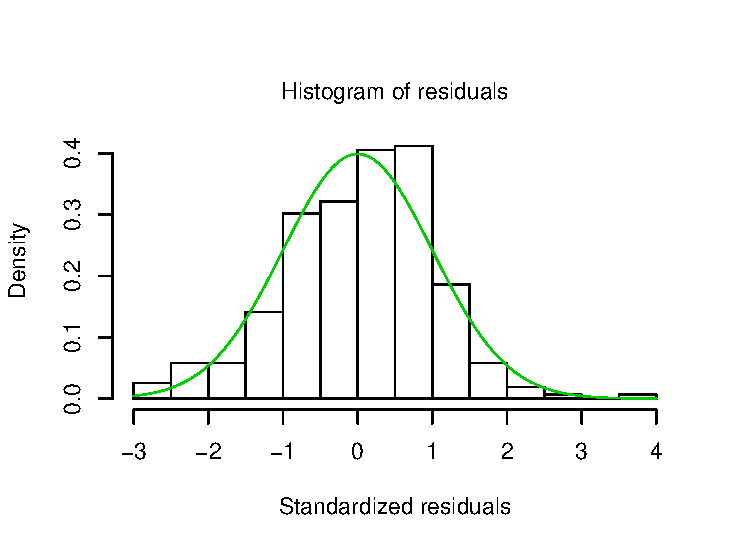
\includegraphics{img/img-unnamed-chunk-6-1} \end{center}

\end{CodeChunk}

\hypertarget{decomposition}{%
\subsection{Decomposition}\label{decomposition}}

As afore-mentioned the decomposition method differs between TRAMO-SEATS+
and X-12ARIMA/X-13ARIMA, where SEATS is based on ARIMA-model and
X11-algorithm on linear filters. Therefore also the composition of this
object differs when estimating with the two methods (hence the two
decomposition objects in the table \ref{tab:obj_tab}). The only common
part is the first two sub-objects with the model specification
(\code{specification}) and information on the decomposition mode
(\code{mode}; e.g.: additive).

Then, the \code{decomposition_X11} object comprises quality measures on
the decomposition (\code{mstats}), namely the \(M\) and \(Q\)
statistics. It contains also the final unmodified S-I ratios \(d8\) and
final seasonal factors \(d10\) (\code{si_ratio}), as well as the
information on the final seasonal filter (\code{s_filter}) and trend
filter(\code{t_filter}). The code below presents the output for X11
decomposition:

\begin{CodeChunk}

\begin{CodeInput}
R> sax13$decomposition
\end{CodeInput}

\begin{CodeOutput}
 Monitoring and Quality Assessment Statistics:  
      M stats
M(1)    0.028
M(2)    0.033
M(3)    0.338
M(4)    0.376
M(5)    0.366
M(6)    0.067
M(7)    0.066
M(8)    0.157
M(9)    0.073
M(10)   0.145
M(11)   0.120
Q       0.156
Q-M2    0.171

Final filters: 
Seasonal filter:  3x5
Trend filter:  13 terms Henderson moving average
\end{CodeOutput}
\end{CodeChunk}

As a reminder, in SEATS it is assumed that each component of the
linearized series (received from TRAMO) is an outcome of a linear
stochastic process and SEATS estimates an ARIMA model for each component
(i.e.~trend, seasonal, transitory and irregular). Subsequently, the
\code{decomposition_SEATS} object contains the information on the
estimated ARIMA models (\code{model}), the linearized components, as
obtained from TRAMO (\code{linearized}), and the theoretical components
calculated from the ARIMA models (\code{components}). The code below
presents the output for the SEATS decomposition, with the information on
the ARIMA models:

\begin{CodeChunk}

\begin{CodeInput}
R> #sats$decomposition
\end{CodeInput}
\end{CodeChunk}

\hypertarget{final}{%
\subsection{Final}\label{final}}

The final object has a simple structure as it includes the input series,
final seasonally adjusted series and the final components (i.e.~\(t\) -
trend-cycle, \(s\) - seasonal component and \(i\) - irregular component)
(\code{series}), as well as their forecasts (\code{forecasts}).

\begin{CodeChunk}

\begin{CodeInput}
R> sats$final
\end{CodeInput}

\begin{CodeOutput}
Last observed values
             y       sa        t             s           i
Jan 2017  96.5 102.9317 102.6366  -6.431739755  0.29515069
Feb 2017  99.3 102.3815 102.7523  -3.081452963 -0.37082579
Mar 2017 110.5 103.2230 103.0587   7.276971010  0.16431902
Apr 2017 103.4 103.3950 103.4579   0.004977088 -0.06292068
May 2017 104.6 104.1023 103.8400   0.497657700  0.26230153
Jun 2017 107.7 103.8403 104.2863   3.859652578 -0.44596785
Jul 2017 107.6 105.1862 104.9032   2.413785110  0.28301107
Aug 2017  88.7 105.5484 105.5999 -16.848375561 -0.05151353
Sep 2017 112.1 106.2889 106.3305   5.811052841 -0.04159101
Oct 2017 113.4 106.9003 107.1101   6.499696169 -0.20982123
Nov 2017 114.3 108.3110 107.7487   5.988950554  0.56232415
Dec 2017 101.7 107.7534 108.1104  -6.053350690 -0.35709913

Forecasts:
               y_f     sa_f      t_f         s_f           i_f
Jan 2018 102.49061 108.4010 108.4016  -5.9103802 -0.0005820963
Feb 2018 105.85284 108.8666 108.7446  -3.0137577  0.1219532717
Mar 2018 116.21918 108.9840 109.0820   7.2351710 -0.0979861094
Apr 2018 108.90762 109.4437 109.4153  -0.5360850  0.0284199810
May 2018 110.11320 109.7634 109.7457   0.3498301  0.0176868066
Jun 2018 114.47710 110.0480 110.0740   4.4290998 -0.0260150048
Jul 2018 112.47723 110.4145 110.4009   2.0627149  0.0136293681
Aug 2018  93.98244 110.7265 110.7267 -16.7440681 -0.0002045225
Sep 2018 116.57469 111.0463 111.0518   5.5283721 -0.0054794124
Oct 2018 118.30580 111.3809 111.3764   6.9249450  0.0044980848
Nov 2018 117.56621 111.6992 111.7005   5.8670241 -0.0013538638
Dec 2018 105.59658 112.0237 112.0245  -6.4271099 -0.0007722619
\end{CodeOutput}
\end{CodeChunk}

\hypertarget{diagnostics}{%
\subsection{Diagnostics}\label{diagnostics}}

This part of the \code{sa_object} includes several diagnostics on the
presence of seasonality in the input series and on the quality of the
seasonal adjustment.

The test for the seasonality presence (\code{combined_test}) are
performed both on the entire series and in the last 3 years.

Whereas, the quality checking is grouped into two sets. The first looks
at the contribution of each estimated component to the variance of the
original series (\code{variance_decomposition}). The second verifies,
with different tests, that there is no seasonal pattern left in the
seasonally adjusted series and in the irregular component
(\code{residuals_test}).

All the checks (except \code{combined_seasonality_test}), together with
a detailed description, are displayed when printing the diagnostics
object.

\begin{CodeChunk}

\begin{CodeInput}
R> #sats$diagnostics
\end{CodeInput}
\end{CodeChunk}

\hypertarget{user-def}{%
\subsection{user defined}\label{user-def}}

As presented in the table \ref{tab:obj_tab} and in the previous sections
the \code{sa_object} has a defined structure with a defined content.
Nevertheless the user can extract additional output from the seasonal
adjustment estimation that will be stored under user\_defined object in
a form of a list. In order extract the additional output the extra
variables need to be defined as characters under the argument
\code{userdefined} of the functions \code{x13_def()},
\code{tramoseats_def()}, \code{x13()} or \code{tramoseats()} (the latter
two functions are presented in the next section \ref{user-def-spec}).

For example, to extract the additional tables \(c10\) and \(d16\) the
following need to be specified in the function argument:

\begin{CodeChunk}

\begin{CodeInput}
R> sa_usrdef <- x13_def(myseries, spec = "RSA3", 
R+                      userdefined = c("decomposition.c10", "decomposition.d16"))
R> sa_usrdef$user_defined
\end{CodeInput}

\begin{CodeOutput}
Names of additional variables (2):
decomposition.c10, decomposition.d16
\end{CodeOutput}
\end{CodeChunk}

The list of all available variables can be extracted with the following
functions:

\begin{itemize}
\item
  \code{user_defined_variables("X13-ARIMA")}
\item
  \code{user_defined_variables("TRAMO-SEATS")}
\end{itemize}

\hypertarget{user-def-spec}{%
\section{Model specification: creation and
modification}\label{user-def-spec}}

The user can also create its own specification, modifying a pre-defined
specification (described in tables \ref{tab:pre_def_ts} and
\ref{tab:pre_def_x13}) or a previously defined specification. For that,
they are two functions for each method (RegARIMA model or seasonal
adjustment with X-13ARIMA or TRAMO-SEATS):

\begin{enumerate}
\def\labelenumi{\arabic{enumi}.}
\item
  One to create a specification from a pre-defined JDemetra+ model
  specification. The corresponding functions are:
  \code{regarima_spec_def_x13()} and
  \code{regarima_spec_def_tramoseats()} for the RegARIMA model, and
  \code{x13_spec_def()} and \code{tramoseats_spec_def()} for the entire
  seasonal adjustment model (including the pre-adjustment with a
  RegARIMA model).
\item
  One to create a specification from a previous specification or a
  model. The corresponding functions are: \code{regarima_spec_x13()} and
  \code{regarima_tramoseats()} for the RegARIMA model, and
  \code{x13_spec()} and \code{tramoseats_spec()} for the entire seasonal
  adjustment model (including the pre-adjustment with a RegARIMA model).
\end{enumerate}

Once the specification is created, the regARIMA model can be performed
by \code{regarima()}, the seasonal adjustment with X-13ARIMA by
\code{x13()} and with TRAMO-SEATS by \code{tramoseats()}.

For example, to create its own RegARIMA model for the TRAMO-SEATS method
by adding an additive outlier in October 2009:

\begin{CodeChunk}

\begin{CodeInput}
R> regarima_ts_spec <- regarima_spec_def_tramoseats(spec = "TRfull",
R+              usrdef.outliersEnabled = TRUE,
R+              usrdef.outliersType = "AO",
R+              usrdef.outliersDate = "2009-10-01")
R> regarima_ts_model <- regarima(series = ipi_c_eu[, "EA19"],
R+                               spec = regarima_ts_spec)
R> regarima_ts_model
\end{CodeInput}

\begin{CodeOutput}
y = regression model + arima (3, 1, 0, 0, 1, 1)
Log-transformation: no
Coefficients:
          Estimate Std. Error
Phi(1)     0.09633      0.055
Phi(2)    -0.16551      0.055
Phi(3)    -0.29422      0.056
BTheta(1) -0.50637      0.051

             Estimate Std. Error
Monday       -0.23323      0.094
Tuesday      -0.01617      0.094
Wednesday     0.29430      0.095
Thursday     -0.35287      0.095
Friday        0.13248      0.094
Saturday      0.30763      0.095
AO (10-2009) -0.80480      0.787
AO (1-2016)   3.25565      0.807


Residual standard error: 1.226 on 311 degrees of freedom
Log likelihood = -506.6, aic =  1039 aicc =  1040, bic(corrected for length) = 0.6292
\end{CodeOutput}
\end{CodeChunk}

And to modify the specification of the x-13ARIMA model of the object
\code{sa_usrdef}, defined in section \ref{user-def}, changing the
seasonal filter and performing a working day adjustment:

\begin{CodeChunk}

\begin{CodeInput}
R> sa_x13_spec <- x13_spec(object = sa_usrdef,
R+                          tradingdays.option = "WorkingDays",
R+                          x11.seasonalma = "S3X3")
R> sa_x13_model <- x13(series = ipi_c_eu[, "EA19"],
R+                     spec = sa_x13_spec)
\end{CodeInput}
\end{CodeChunk}

Almost all the specification variables available in JDemetra+ can be
used in \pkg{RJDemetra}\footnote{In the current release of the package,
  it is not possible to use user-defined calendars regressors: they have
  to be added as user-defined variable (the difference is that there is
  no automatic test to remove or not the regressors). Moreover, contrary
  to what is possible under JDemetra+, ramp effects and intervention
  variables are not intended to be added in the specification since the
  corresponding regressors can be easily created through \proglang{R}.}.
For more details see the help of the corresponding function or the
documentation of JDemetra+.

To prevent from wrong user-defined specification, they are also
automatic checks in \pkg{RJDemetra}, like in JDemetra+. For example, to
pre-specify an outlier or a user-defined variable you have to enable
them (setting the parameter \code{usrdef.outliersEnabled} or
\code{usrdef.varEnabled} to \code{TRUE}); or to fix the coefficient of
an outlier or a user-defined regressor you have to specify the
transformation function (\code{transform.function}, it cannot be
automatic). Those checks are done each time a new specification is
create. Therefore, some specifications cannot be set in two stages. For
example, fixing the coefficient of an outlier has to be done at the same
time when the outliers are defined. The following code doesn't fix the
coefficient of the outlier previously in January 2001:

\begin{CodeChunk}

\begin{CodeInput}
R> regarima_wrong_spec <- regarima_spec_tramoseats(object = regarima_ts_model,
R+              transform.function = "Log",
R+              usrdef.outliersCoef =  -0.8)
\end{CodeInput}
\end{CodeChunk}

To fix it you have to re-defined the outlier:

\begin{CodeChunk}

\begin{CodeInput}
R> regarima_good_spec <- regarima_spec_tramoseats(object = regarima_ts_model,
R+              transform.function = "Log",
R+              usrdef.outliersType = "AO",
R+              usrdef.outliersDate = "2009-10-01",
R+              usrdef.outliersCoef =  -0.8)
\end{CodeInput}
\end{CodeChunk}

The documentation for the functions modifying specifications provide
information on the interdependencies between different arguments. The
package offers also functions to display different part of the model
specification. These are presented under the entry \code{specification}
of the package documentation. For instance, from the example above, we
can check which user defined variables were enabled and with which
parameters.

In the first case (wrongly specified), an outlier was pre-defined but
its coefficient was not fixed:

\begin{CodeChunk}

\begin{CodeInput}
R> s_usrdef(regarima_wrong_spec)
\end{CodeInput}

\begin{CodeOutput}
 outlier outlier.coef variables variables.coef
    TRUE        FALSE     FALSE          FALSE
\end{CodeOutput}

\begin{CodeInput}
R> s_preOut(regarima_wrong_spec)
\end{CodeInput}

\begin{CodeOutput}
  type       date coeff
1   AO 2009-10-01    NA
\end{CodeOutput}
\end{CodeChunk}

In the second case, the coefficient was correctly fixed:

\begin{CodeChunk}

\begin{CodeInput}
R> s_usrdef(regarima_good_spec)
\end{CodeInput}

\begin{CodeOutput}
 outlier outlier.coef variables variables.coef
    TRUE         TRUE     FALSE          FALSE
\end{CodeOutput}

\begin{CodeInput}
R> s_preOut(regarima_good_spec)
\end{CodeInput}

\begin{CodeOutput}
  type       date coeff
1   AO 2009-10-01  -0.8
\end{CodeOutput}
\end{CodeChunk}

\hypertarget{manipulate-workspace}{%
\section{Manipulate JDemetra+ workspaces}\label{manipulate-workspace}}

\pkg{RJDemetra} allows to interact with JDemetra+ workspace that can be
openned by the software. A workspace includes:

\begin{itemize}
\tightlist
\item
  The XML file that enables the user to import the workspace to
  JDemetra+ and to display it content;\\
\item
  A folder containing several sub-folfders that correspond to the
  different types of items created by the user.
\end{itemize}

Each workspace can contain several multi-processings and each
multi-processing stores the results of the seasonal adjustment procedure
performed with the TRAMO-SEATS or X-13ARIMA-SEATS methods.

Export models to workspace allows to store easily the seasonal
adjustment models, to change the specifications with the JDemetra+
graphical interface and to give models users unfamiliar with
\proglang{R}.

\hypertarget{export-wk}{%
\subsection{Export a workspace}\label{export-wk}}

Four functions have to be used to export models:

\begin{itemize}
\tightlist
\item
  \code{new_workspace()} to create a workspace;\\
\item
  \code{new_multiprocessing()} to create a multi-processing in a
  workspace;\\
\item
  \code{add_sa_item()} to add a seasonal adjustment model to a
  multi-processing;\\
\item
  \code{save_workspace()} to export the workspace.
\end{itemize}

The following command export the seasonal adjustment models compute by
TRAMO-SEATS+ and X-13ARIMA-SEATS:

\begin{CodeChunk}

\begin{CodeInput}
R> myseries <- ipi_c_eu[, "EA19"]
R> sa_x13 <- x13_def(myseries)
R> sa_ts <- tramoseats_def(myseries)
\end{CodeInput}
\end{CodeChunk}

To create a workspace and a multi-processing names ``MP-1'':

\begin{CodeChunk}

\begin{CodeInput}
R> wk <- new_workspace()
R> new_multiprocessing(wk, name = "MP-1")
\end{CodeInput}
\end{CodeChunk}

The two models will be added in the multiprocessing ``MP1'': the name of
the seasonal adjustment model computed with X-13ARIMA-SEATS will be ``SA
with X13'' and the one with TRAMO-SEATS+ will be ``SA with TramoSeats'':

\begin{CodeChunk}

\begin{CodeInput}
R> add_sa_item(wk, multiprocessing = "MP-1",
R+             sa_obj = sa_x13, name =  "SA with X13")
R> add_sa_item(wk, multiprocessing =  "MP-1",
R+             sa_obj = sa_ts, name = "SA with TramoSeats")
\end{CodeInput}
\end{CodeChunk}

The workspace exported is named ``workspace.xml'':

\begin{CodeChunk}

\begin{CodeInput}
R> save_workspace(wk, file =  "workspace.xml")
\end{CodeInput}
\end{CodeChunk}

\hypertarget{import-a-workspace}{%
\subsection{Import a workspace}\label{import-a-workspace}}

Height functions can be used to import a workspace:

\begin{itemize}
\tightlist
\item
  \code{load_workspace()} to load a workspace;\\
\item
  \code{compute()} to compute the multi-processings: by default a
  workspace only contains definitions, computation is needed to get the
  seasonal adjustment model;\\
\item
  \code{get_model()} to get the seasonal adjusted models;\\
\item
  \code{get_ts()} to get the input raw time series, \code{get_object()}
  and \code{get_all_objects} to navigate inside the workspace (extract a
  multi-processing or a seasonal adjustment model), \code{get_name()} to
  get the names of the multiprocessings or the seasonal adjustment
  models and \code{count()} to count the number of multiprocessing or
  seasonal adjustment models.
\end{itemize}

For instance, to import the workspace created in section \ref{export-wk}
and to get the first multiprocessing and the first seasonal adjustment
model:

\begin{CodeChunk}

\begin{CodeInput}
R> wk <- load_workspace(file =  "workspace.xml")
R> mp1 <- get_object(wk, 1)
R> sa_item1 <- get_object(mp1, 1)
\end{CodeInput}
\end{CodeChunk}

To get the number of seasonal adjustment models in the multiprocessing:

\begin{CodeChunk}

\begin{CodeInput}
R> count(mp1)
\end{CodeInput}

\begin{CodeOutput}
[1] 2
\end{CodeOutput}
\end{CodeChunk}

And the name of the first seasonal adjustment model in JDemetra+:

\begin{CodeChunk}

\begin{CodeInput}
R> get_name(sa_item1) 
\end{CodeInput}

\begin{CodeOutput}
[1] "SA with X13"
\end{CodeOutput}
\end{CodeChunk}

Raw time series and seasonal adjustment model can now be imported:

\begin{CodeChunk}

\begin{CodeInput}
R> raw_ts <- get_ts(sa_item1)
R> compute(wk)
R> sa_model1 <- get_model(sa_item1, workspace = wk)
\end{CodeInput}
\end{CodeChunk}

\code{get_ts()} and \code{get_model()} can also be used directly to the
workspace or a multiprocessing to import all the raw time series or all
the seasonal adjustment model:

\begin{itemize}
\tightlist
\item
  for a multiprocessing the result is a list which each element contains
  the information of a seasonal adjustment model;\\
\item
  for a workspace the result is a list of length the number of
  multi-processing and which each element contains a list with the
  information of each seasonal adjustment model.
\end{itemize}

For example to get all raw time series of the workspace and all seasonal
adjustmen models of the first multi-processing:

\begin{CodeChunk}

\begin{CodeInput}
R> all_raw_ts <- get_ts(wk)
R> sa_models_of_mp1 <- get_model(mp1, workspace = wk)
\end{CodeInput}
\end{CodeChunk}

The imports of seasonal adjustment models from a workspace works well
when it has been created throw \pkg{RJDemetra}. They may be some
troubles when importing a workspace created with JDemetra+, in
particular:

\begin{itemize}
\tightlist
\item
  \pkg{RJDemetra} doesn't support yet user-defined calendars. A seasonal
  adjustment model defined with a specific calendar or user-defined
  calendar regressors will be partially imported. The result will be
  correct but changing the specification (throw \code{x13_spec()} or
  \code{tramoseats_spec()}) will erase user-defined calendars.\\
\item
  Seasonal adjustment models with ramp effect or intervention variables
  will be partially imported: the result of the imported model will be
  correct but changing the specification (throw \code{x13_spec()} or
  \code{tramoseats_spec()}) will erase them.\\
\item
  Seasonal adjustment models with no pre-processing (X-11 specification)
  are not supported: \code{NULL} object will be returned.
\end{itemize}

\hypertarget{conclusion}{%
\section{Conclusion}\label{conclusion}}

\hypertarget{acknowledgments}{%
\section{Acknowledgments}\label{acknowledgments}}

\renewcommand\refname{References}
\bibliography{biblio.bib}


\end{document}

